\documentclass{beamer}
\usepackage[utf8]{inputenc}

\usetheme{Madrid}
\usecolortheme{default}
\usepackage{amsmath,amssymb,amsfonts,amsthm}
\usepackage{txfonts}
\usepackage{tkz-euclide}
\usepackage{listings}
\usepackage{adjustbox}
\usepackage{array}
\usepackage{tabularx}
\usepackage{gvv}
\usepackage{lmodern}
\usepackage{circuitikz}
\usepackage{tikz}
\usepackage{graphicx}

\setbeamertemplate{page number in head/foot}[totalframenumber]

\usepackage{tcolorbox}
\tcbuselibrary{minted,breakable,xparse,skins}



\definecolor{bg}{gray}{0.95}
\DeclareTCBListing{mintedbox}{O{}m!O{}}{%
  breakable=true,
  listing engine=minted,
  listing only,
  minted language=#2,
  minted style=default,
  minted options={%
    linenos,
    gobble=0,
    breaklines=true,
    breakafter=,,
    fontsize=\small,
    numbersep=8pt,
    #1},
  boxsep=0pt,
  left skip=0pt,
  right skip=0pt,
  left=25pt,
  right=0pt,
  top=3pt,
  bottom=3pt,
  arc=5pt,
  leftrule=0pt,
  rightrule=0pt,
  bottomrule=2pt,
  toprule=2pt,
  colback=bg,
  colframe=orange!70,
  enhanced,
  overlay={%
    \begin{tcbclipinterior}
    \fill[orange!20!white] (frame.south west) rectangle ([xshift=20pt]frame.north west);
    \end{tcbclipinterior}},
  #3,
}
\lstset{
    language=C,
    basicstyle=\ttfamily\small,
    keywordstyle=\color{blue},
    stringstyle=\color{orange},
    commentstyle=\color{green!60!black},
    numbers=left,
    numberstyle=\tiny\color{gray},
    breaklines=true,
    showstringspaces=false,
}
\title{2.4.43}
\date{22nd August, 2025}
\author{Puni Aditya - EE25BTECH11046}

\begin{document}

\frame{\titlepage}
\begin{frame}{Question}
Show that the lines $\frac{x-5}{7}=\frac{y+2}{-5}=\frac{z}{1}$ and $\frac{x}{1}=\frac{y}{2}=\frac{z}{3}$ are perpendicular to each other.
\end{frame}

\begin{frame}{allowframebreaks}
\frametitle{Equation}
For the two lines to be perpendicular, the inner product or dot product of their direction vectors must be zero.
\begin{align}
    \vec{d_1}^\top \vec{d_2} = 0 \label{eq:1}
\end{align}
From the equations of the lines $L_1$ and $L_2$,
\begin{align}
    \vec{d_1} = \myvec{7 \\ -5 \\ 1}, 
    \vec{d_2} = \myvec{1 \\ 2 \\ 3}
\end{align}
\end{frame}

\begin{frame}{Theoretical Solution}
From \ref{eq:1},
\begin{align}
    \vec{d_1}^\top \vec{d_2} &= \myvec{7&-5&1}\myvec{1 \\ 2 \\ 3} \\
    &= \brak{7}\brak{1} + \brak{-5}\brak{2} + \brak{1}\brak{3} \\
    &= 7 - 10 + 3 \\
    &= 0
\end{align}

$\because$ The dot product of the direction vectors of the two lines is 0 \\
$\implies$ The lines are \textbf{perpendicular} to each other.
\end{frame}

\begin{frame}{Plot}
    \begin{figure}
    \centering
    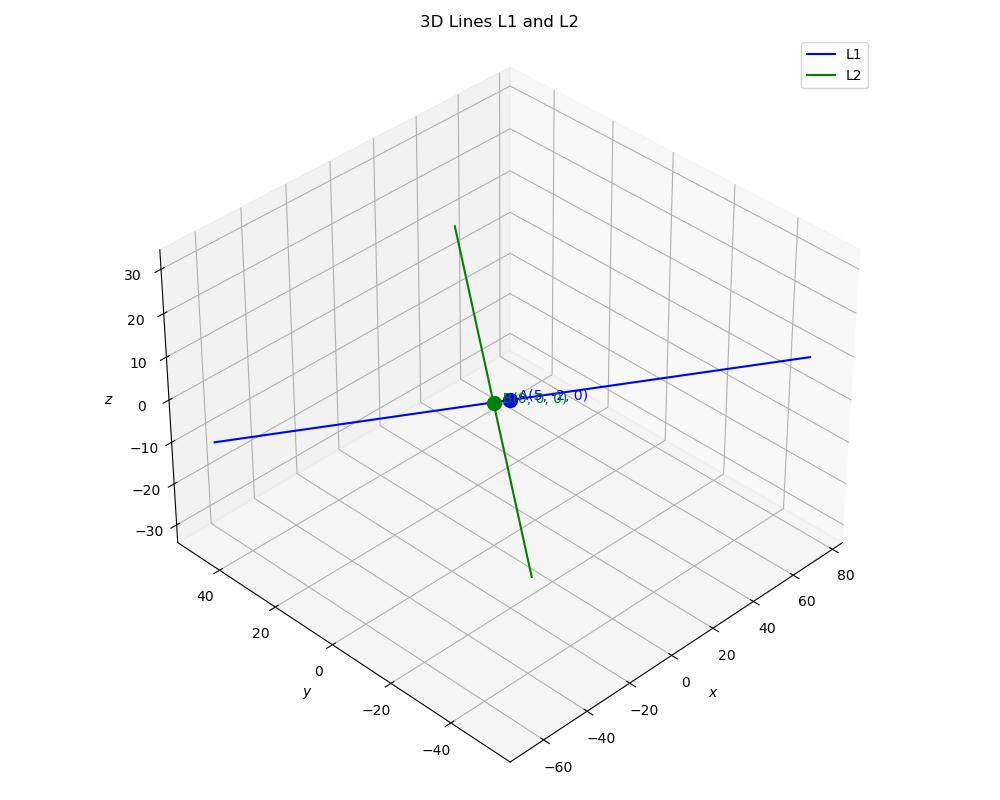
\includegraphics[width=0.5\columnwidth]{../figs/plot_c.jpg}
    \caption{Lines $L_1$ and $L_2$}
    \label{fig:fig}
\end{figure}
\end{frame}

\end{document}
